\section{Auswertung}


\subsection{Untersuchung der Charakteristik des Zählrohres}
Die aufgenommen Messwerte für die Zählrate $N$ unter variabler Betriebspspannung $U$ sind
in Tabelle \ref{tab: zaelrate_strom} aufgeführt. Der angegebene Fehler wurde hierbei stets
auf eine ganze Zahl gerundet. Eine Darstellung der Messwerte befindet sich in Abbildung \ref{fig: zählrate_ges}.
Als obere und untere Schranke für die Betrachtung des Plateaus wurden die Werte zwischen $U = \SI{370}{\volt}$
und $U = \SI{600}{\volt}$ gewählt, da an den Grenzen dieses Intervalls ein signifikanter Unterschied zu einem
linearen Verlauf zu erkennen ist (vgl. die beiden benachbarten Werte in Abbildung \ref{}). Mittels linearer
Regressionsrechnung ergeben sich für die Steigung $m$ und den Ordinatenabschnitt $b$ folgende Werte
\begin{align}
  m &= \SI{0.041 \pm 0.009}{\per\second\per\volt} \\
  b &= \SI{412 \pm 4}{\per\second}
\end{align}
Eine graphische Darstellung der Messwerte im gewählten Plateaubereich, sowie die Regressiongerade sind in
Abbildung \ref{fig: plateau} einzusehen.

\subsection{Bestimmung der Totzeit}
Mit Hilfe des Oszilloskops wurde die Totzeit fünf mal unter verschiedenen Betriebsspannungen ausgemessen. Die Messwerte
sind in Tabelle \ref{} aufgetragen. Für den Mittelwert mit zugehöriger Standardabweichung ergibt sich
\begin{equation}
  T_1 = \SI{96 \pm 2}{\micro\second}.
\end{equation}
\begin{table} 
\centering 
\caption{Mit dem Oszilloskop gemessene Totzeiten $T$ unter verschiedenen Beschleunigungsspannungen $U$.} 
\label{tab: totzeit_oszi} 
\begin{tabular}{S S } 
\toprule  
{$U/ \si{\volt}$} & {$T/ \si{\micro\second}$}  \\ 
\midrule  
 360  & 100\\ 
400  & 90\\ 
460  & 90\\ 
500  & 100\\ 
540  & 100\\ 
\bottomrule 
\end{tabular} 
\end{table}

\begin{table} 
\centering 
\caption{Mit dem Oszilloskop gemessene Erholungszeiten $T_E$ unter verschiedenen Beschleunigungsspannungen $U$.} 
\label{tab: erholungszeit} 
\begin{tabular}{S S } 
\toprule  
{$U/ \si{\volt}$} & {$T_E/ \si{\micro\second}$}  \\ 
\midrule  
 520  & 300\\ 
540  & 250\\ 
570  & 250\\ 
630  & 300\\ 
640  & 300\\ 
\bottomrule 
\end{tabular} 
\end{table}


\newpage
\input{table/zählrate_strom.tex}
\begin{figure}
  \centering
  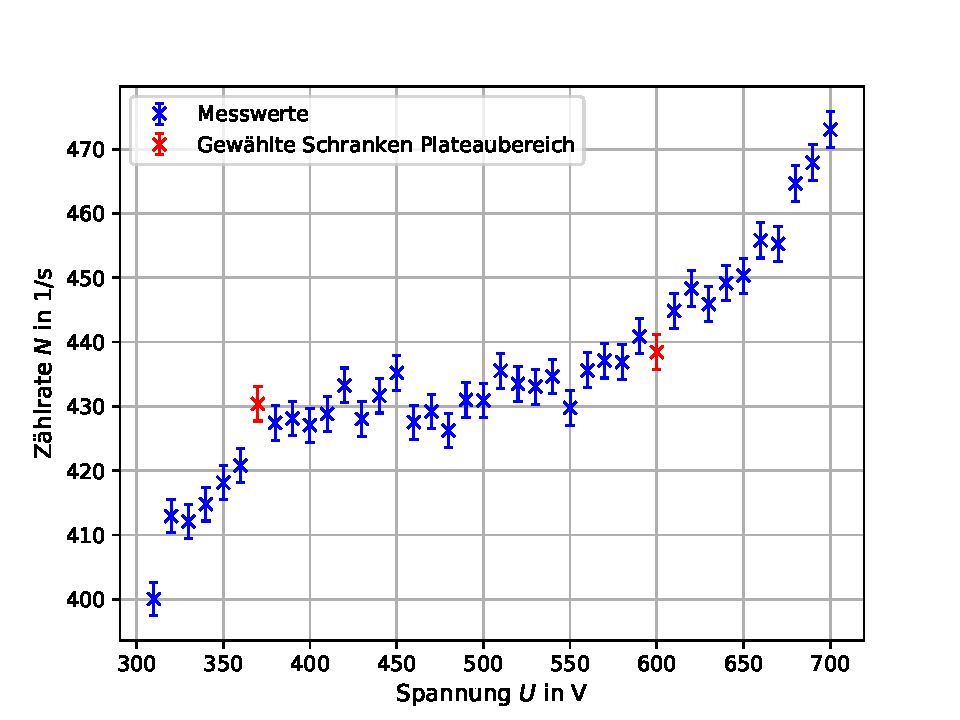
\includegraphics[width = 0.8\textwidth]{../Messdaten/plots/all_counts.pdf}
  \caption{Graphische Darstellung der Zählrohrcharakteristik, Abhängigkeit der Zählrate $N$ von der Betriebsspannung $U$.}
  \label{fig: zählrate_ges}
\end{figure}
\begin{figure}
  \centering
  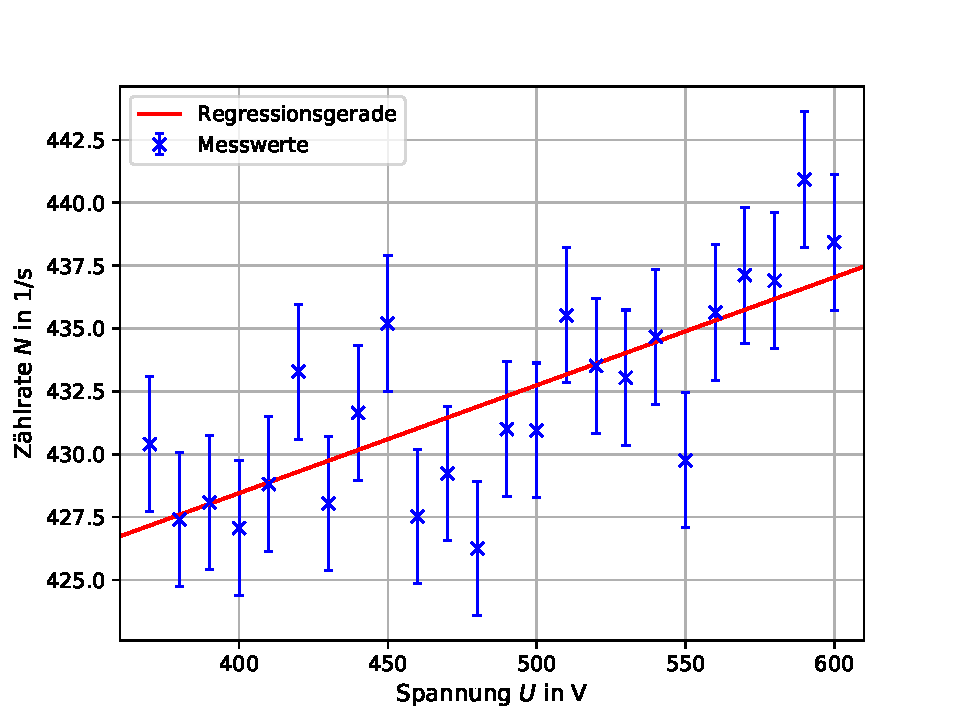
\includegraphics[width = 0.8\textwidth]{../Messdaten/plots/plateau.pdf}
  \caption{Graphische Darstellung des Plateaubereichs.}
  \label{fig: plateau}
\end{figure}
